\begin{figure}[H]
  \centering
  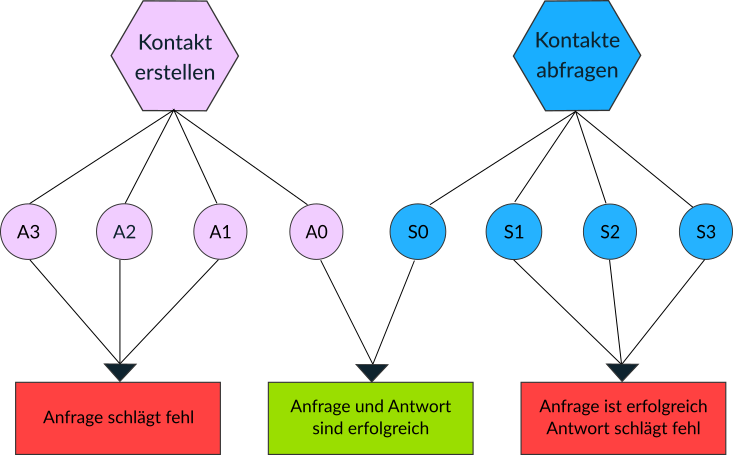
\includegraphics[width=0.8\textwidth]{Szenarien}
  \grayRule
  \caption{Szenarien bei der Datenübertragung über das Netzwerk}
  \label{fig:szenarien}
\end{figure}
% \todo{Erstellen = erstellen, aktualisieren, löschen}
\begin{description}[leftmargin=0.5cm,style=nextline]
% client push
\item[Szenario A0:]
Der Client erstellt einen Adressbucheintrag, hat den Status \sc{online} und der Server ist erreichbar. Sowohl Anfrage als auch Antwort ist erfolgreich. Der Kontakt wird erfolgreich erstellt.\\
\item[Szenario A1:]
Der Client erstellt einen Adressbucheintrag, hat den Status \sc{offline} und der Server ist nicht erreichbar. Die Anfrage schlägt fehl.\\
\item[Szenario A2:]
Der Client erstellt einen Adressbucheintrag und hat den Status \sc{online}. Die Anfrage wird gestartet und währenddessen bricht die Internetverbindung ab. Die Anfrage `wartet` bis ein Timeout getriggert wird und schlägt dann fehl. Wärend des Wartens ist der Client blockiert.\\
\item[Szenario A3:]
Der Client erstellt einen Adressbucheintrag und hat den Status \sc{online}. Die Anfrage wird gestartet und währenddessen bricht die Internetverbindung ab. Die Anfrage ist teilweise erfolgreich. Nur ein Teil der Telefonnummer kommen beim Server an.\\
% client pull / server push
\item[Szenario S0:]
Der Client fordert eine Liste aller gespeicherten Kontakte vom Server an, hat den Status \sc{online} und der Server ist erreichbar. Sowohl Anfrage als auch Antwort ist erfolgreich. Die Liste wird komplett ausgeliefert.\\
\item[Szenario S1:]
Der Client fordert eine Liste aller gespeicherten Kontakte vom Server an, hat den Status \sc{offline} und der Server ist nicht erreichbar. Die Antwort schlägt fehl.\\
\item[Szenario S2:]
Der Client fordert eine Liste aller gespeicherten Kontakte vom Server an und hat den Status \sc{online}. Während der Server antwortet bricht die Internetverbindung ab. Die Antwort `wartet` bis ein Timeout getriggert wird schlägt dann fehl. Wärend des Wartens ist der Client blockiert.\\
\item[Szenario S3:]
Der Client fordert eine Liste aller gespeicherten Kontakte vom Server an und hat den Status \sc{online}. Während der Server antwortet bricht die Internetverbindung ab. Die Antwort ist teilweise erfolgreich. Nur ein Teil der angefragten Daten kommen beim Client an.
\end{description}
In den obigen Szenarien wird nicht beschrieben warum die Internetverbindung abbricht. Dies kann verschiedene Gründe haben. Um nur einige Beispiele zu nennen: Eine langsame Internetverbindung, oder eine Fahrt durch einen Tunnel kann ein Timeout während einer Aktion hervorrufen. Ein auf einer Baustelle gekapptes Kabel oder ein Stromausfall kann zu zeitweise vollständigen Internetverlust (haha) führen.
%
% ERGEBNIS
%
\subsubsection*{Ergebnis}
Da die Szenarien \it{A0} und \it{S0}, die Szenarien \it{A1}, \it{A2} und \it{A3} sowie die Szenazien \it{S1}, \it{S2} und \it{S3} zusammengefasst werden können, ergeben sich aus den acht Szenarien die drei nun aufgezählten Fälle.
\begin{itemize}
  \item Fall a: Anfrage und Antwort sind erfolgreich.
  \item Fall b: Anfrage ist nicht erfolgreich
  \item Fall c: Anfrage ist erfolgreich, Antwort schlägt fehl
\end{itemize}